\documentclass[a4paper]{article}
\usepackage{a4wide,amssymb,epsfig,latexsym,multicol,array,hhline,fancyhdr}
\usepackage[utf8]{vntex, inputenc}
\usepackage[english]{babel}
\usepackage{amsmath}
\usepackage{lastpage}
\usepackage[lined,boxed,commentsnumbered]{algorithm2e}
\usepackage{enumerate}
\usepackage{color}
\usepackage{graphicx}							% Standard graphics package
\usepackage{array}
\usepackage{tabularx, caption}
\usepackage{multirow}
\usepackage{multicol}
\usepackage{rotating}
\usepackage{graphics}
\usepackage{geometry}
\usepackage{setspace}
\usepackage{epsfig}
\usepackage{tikz}
\usetikzlibrary{arrows,snakes,backgrounds}
\usepackage{hyperref}
\usepackage{indentfirst}
\usepackage{gensymb}
\usepackage{float}
\hypersetup{urlcolor=blue,linkcolor=black,citecolor=black,colorlinks=true}
%\usepackage{pstcol} 								% PSTricks with the standard color package

\newtheorem{theorem}{{\bf Theorem}}
\newtheorem{property}{{\bf Property}}
\newtheorem{proposition}{{\bf Proposition}}
\newtheorem{corollary}[proposition]{{\bf Corollary}}
\newtheorem{lemma}[proposition]{{\bf Lemma}}

\AtBeginDocument{\renewcommand*\contentsname{Contents}}
\AtBeginDocument{\renewcommand*\refname{References}}
%\usepackage{fancyhdr}
\setlength{\headheight}{40pt}
\pagestyle{fancy}
\fancyhead{} % clear all header fields
\fancyhead[L]{
  \begin{tabular}{rl}
    \begin{picture}(25,15)(0,0)
    \put(0,-8){
\includegraphics[width=8mm, height=8mm]{hcmut.png}}
    %\put(0,-8){\epsfig{width=10mm,figure=hcmut.eps}}
    \end{picture}
	%
\includegraphics[width=8mm, height=8mm]{hcmut.png} & %
    \begin{tabular}{l}
      \textbf{\bf \ttfamily University of Technology, Ho Chi Minh City}\\
      \textbf{\bf \ttfamily Faculty of Computer Science and Engineering}
    \end{tabular}
  \end{tabular}
}
\fancyhead[R]{
	\begin{tabular}{l}
		\tiny \bf \\
		\tiny \bf
	\end{tabular}  }
\fancyfoot{} % clear all footer fields
\fancyfoot[L]{\scriptsize \ttfamily Assignment for Mathematical Modeling\textendash{}Academic year 2020\textendash{}2021}
\fancyfoot[R]{\scriptsize \ttfamily Page {\thepage}/\pageref{LastPage}}
\renewcommand{\headrulewidth}{0.3pt}
\renewcommand{\footrulewidth}{0.3pt}


%%%
\setcounter{secnumdepth}{4}
\setcounter{tocdepth}{3}
\makeatletter
\newcounter{subsubsubsection}[subsubsection]
\renewcommand\thesubsubsubsection{\thesubsubsection.\@alph\c@subsubsubsection}
\newcommand\subsubsubsection{\@startsection{subsubsubsection}{4}{\z@}%
                                     {-3.25ex\@plus-1ex \@minus-.2ex}%
                                     {1.5ex \@plus.2ex}%
                                     {\normalfont\normalsize\bfseries}}
\newcommand*\l@subsubsubsection{\@dottedtocline{3}{10.0em}{4.1em}}
\newcommand*{\subsubsubsectionmark}[1]{}
\makeatother

\everymath{\color{blue}}

\begin{document}

\begin{titlepage}
  \begin{center}
    VIETNAM NATIONAL UNIVERSITY, HO CHI MINH CITY \\
    UNIVERSITY OF TECHNOLOGY \\
    FACULTY OF COMPUTER SCIENCE AND ENGINEERING
  \end{center}

  \vspace{1cm}

  \begin{figure}[h!]
    \begin{center}
      
\includegraphics[width=3cm]{hcmut.png}
    \end{center}
  \end{figure}

  \vspace{1cm}


  \begin{center}
    \begin{tabular}{c}
      \multicolumn{1}{l}{\textbf{{\Large MATHEMATICAL MODELING  (CO2011)}}}               \\
      {}                                                                                  \\
      \hline
      \\
      \multicolumn{1}{l}{\textbf{{\Large Assignment (Semester 201, Duration: 06 weeks)}}} \\
      \\
      \textbf{{\Huge Dynamical systems in forecasting}}                                   \\
      \\
      \textbf{{\Huge Greenhouse Micro-climate}}                                           \\
      \\
      \hline
    \end{tabular}
  \end{center}

  \vspace{3cm}

  \begin{table}[h]
    \begin{tabular}{rrl}
      \hspace{5 cm} & Advisor: & Nguyễn Tiến Thịnh \\
                    &          & Nguyễn An Khương  \\
                    & TA:      & Trần Trung Hiếu   \\
    \end{tabular}
  \end{table}

  \begin{center}
    {\footnotesize HO CHI MINH CITY, DECEMBER 2020}
  \end{center}
\end{titlepage}


%\thispagestyle{empty}

\newpage
\tableofcontents
\newpage


%%%%%%%%%%%%%%%%%%%%%%%%%%%%%%%%%
\section*{Member list \& Workload}

\begin{center}
  \begin{tabular}{|c|c|c|l|c|}
    \hline
    \textbf{No.}       & \textbf{Fullname}                      & \textbf{Student ID}      & \textbf{Problems}                             & \textbf{Percentage of work} \\
    \hline
    %%%%%Student 1%%%%%%%%%%
    \multirow{3}{*}{1} & \multirow{3}{*}{Lưu Nguyễn Hoàng Minh} & \multirow{3}{*}{1952845} & \textendash{} Relation \& Counting: 1, 2, 3   & \multirow{3}{*}{20\%}       \\
                       &                                        &                          & Bonus: 1, 2, 3.                               &                             \\
                       &                                        &                          & \textendash{} Probability: 1, 2, 3.           &                             \\
    \hline
    %%%%%Student 2%%%%%%%%%%%
    \multirow{3}{*}{2} & \multirow{3}{*}{Vũ Anh Nhi}            & \multirow{3}{*}{1952380} & \textendash{} Relation \& Counting: 4, 5, 6   & \multirow{3}{*}{20\%}       \\
                       &                                        &                          & Bonus: 4, 5, 6.                               &                             \\
                       &                                        &                          & \textendash{} Graph: 1, 2, 3, Bonus: 1, 2, 3. &                             \\
    \hline
    %%%%%Student 3%%%%%%%%%%%
    \multirow{3}{*}{3} & \multirow{3}{*}{Nguyễn Phú Nghĩa}      & \multirow{3}{*}{1952355} & \textendash{} Relation \& Counting: 4, 5, 6   & \multirow{3}{*}{20\%}       \\
                       &                                        &                          & Bonus: 4, 5, 6.                               &                             \\
                       &                                        &                          & \textendash{} Graph: 1, 2, 3, Bonus: 1, 2, 3. &                             \\
    \hline
    %%%%%Student 4%%%%%%%%%%%
    \multirow{3}{*}{4} & \multirow{3}{*}{Nguyễn Chính Khôi}     & \multirow{3}{*}{1952793} & \textendash{} Relation \& Counting: 4, 5, 6   & \multirow{3}{*}{20\%}       \\
                       &                                        &                          & Bonus: 4, 5, 6.                               &                             \\
                       &                                        &                          & \textendash{} Graph: 1, 2, 3, Bonus: 1, 2, 3. &                             \\
    \hline
    %%%%%Student 5%%%%%%%%%%%
    \multirow{3}{*}{5} & \multirow{3}{*}{Nguyễn Hoàng}          & \multirow{3}{*}{1952255} & \textendash{} Relation \& Counting: 4, 5, 6   & \multirow{3}{*}{20\%}       \\
                       &                                        &                          & Bonus: 4, 5, 6.                               &                             \\
                       &                                        &                          & \textendash{} Graph: 1, 2, 3, Bonus: 1, 2, 3. &                             \\
    \hline
  \end{tabular}
\end{center}


\newpage
%%%%%%%%%%%%%%%%%%%%%%%%%%%%%%%%%
\section{Background}
\subsection{A brief about dynamical systems}
A dynamical system is any system that evolves or changes with respect to time according to some rules.
A state space, also called the phase space, is a model used within dynamical systems to capture these changes.
For investigating dynamical systems, it is necessary to specify some characteristics that provide a subdivision into special classes of dynamical systems.

Dynamical systems are often classified as continuous or discrete.
Continuous systems (also called flows) are given by differential equations.
In such systems, the time intervals between measurements are negligibly small, making changes appear as one long continuum.
Then there are discrete systems (also called maps), which are specified by difference equations.

Another important characteristic of a dynamical system is whether it is time dependent or not.
For time-dependent systems, the function that specifies \(\dot{x}\) or \(\Delta{x_n}\) depends on the time itself, whereas in time-independent systems, this function does not change.

For the analysis, it is important whether a dynamical system is linear or not.
Linear dynamical systems are simple to analyze, unlike non-linear systems, which typically have intricate dynamical behavior.

A general dynamical system contains 2 elements: the initial state and a function or functions describing the next state.
We can choose any point in the state space to be the origin, then depending on the requirements, our functions can be differential or difference.
\begin{equation*}
  \begin{cases}
    a_0           & = C \\
    \frac{da}{dt} & = f
  \end{cases}
\end{equation*}
or
\begin{equation*}
  \begin{cases}
    a_0       & = C       \\
    a_{n + 1} & = a_n + X
  \end{cases}
\end{equation*}
with \(f\) is an arbitrary function or functions, \(C\) and \(X\) are arbitrary variables.

In this assignment, we are required to design first-order differential systems to predict the climate inside an arbitrary greenhouse.
The main climatic components of a greenhouse include temperature, vapor pressure of water and the \(CO_2\) concentration.
These components are are normally affected by one or many elements presented inside the greenhouse, thus we will express these components in terms of differential equations.
\begin{itemize}
  \item Temperature
        \begin{multline*}
          cap_{Can}\dot{T_{Can}} = {}R_{PAR\_SunCan} + R_{NIR\_SunCan} + R_{PipeCan} \\
          - H_{CanAir} - L_{CanAir} - R_{CanCov,in} \\
          - R_{CanFlr} - R_{CanSky} - R_{CanThScr} ~~~~ [W\;m^{-2}]
        \end{multline*}
        \begin{multline*}
          cap_{Air}\dot{T_{Air}} = H_{CanAir} + H_{PadAir} + H_{MechAir} + H_{PipeAir} \\
          + H_{PadAir} + H_{BlowAir} + R_{Glob\_SunAir} \\
          - H_{AirFlr} - H_{AirThScr} - H_{AirOut} \\
          - H_{AirTop} - H_{AirOut\_Pad} - L_{AirFog} ~~~~ [W\;m^{-2}]
        \end{multline*}
        \begin{multline*}
          cap_{Flr}\dot{T_{Flr}} = H_{AirFlr} + R_{PAR\_SunFlr} + R_{NIR\_SunFlr} + R_{CanFlr} + R_{PipeFlr} \\
          - H_{FlrSo1} - R_{FlrCov,in} - R_{FlrSky} - R_{FlrThScr} ~~~~ [W\;m^{-2}]
        \end{multline*}
        \begin{multline*}
          cap_{So(j)}T_{So(j)} = H_{So(j-1)So_{(j)}} - H_{So(j)So(j+1)} ~~~~~~~~~~~~~~~~ j=1,2\dots5 ~~~~ [W\;m^{-2}]
        \end{multline*}
        \begin{multline*}
          cap_{ThScr}\dot{T_{ThScr}} = H_{AirThScr} + L_{AirThScr} \\
          + R_{CanThScr} + R_{FlrThScr} + R_{PipeThScr} \\
          - H_{ThScrTop} - R_{ThScrCov,in} - R_{ThScrSky} ~~~~ [W\;m^{-2}]
        \end{multline*}
        \begin{multline*}
          cap_{Top}\dot{T_{Top}} = H_{ThScrTop} + H_{AirTop} - H_{TopCov,in} - H_{TopOut} ~~~~~~~~~~~~~~~~ [W\;m^{-2}]
        \end{multline*}
        \begin{multline*}
          cap_{Cov,in}\dot{T_{Cov,in}} = H_{TopCov,in} + L_{TopCov,in} + R_{CanCov,in} + R_{FlrCov,in} \\
          + R_{PipeCov,in} + R_{ThScrCov,in} - H_{Cov,inCov,e} ~~~~ [W\;m^{-2}]
        \end{multline*}
        \begin{multline*}
          cap_{Cov,e}\dot{T_{Cov,e}} = R_{Glob\_SunCov} + H_{Cov,inCov,e} - H_{Cov,eOut} - R_{Cov,eSky} ~~~~ [W\;m^{-2}]
        \end{multline*}
        \begin{multline*}
          cap_{Pipe}\dot{T_{Pipe}} = H_{BoilPipe} + H_{IndPipe} + H_{GeoPipe} \\
          - R_{PipeSky} - R_{PipeCov,in} - R_{PipeCan} \\
          - R_{PipeFlr} - R_{PipeThScr} - H_{PipeAir} ~~~~ [W\;m^{-2}]
        \end{multline*}
  \item Vapor pressure
        \begin{multline*}
          cap_{VP_{Air}}\dot{VP_{Air}} = MV_{CapAir} + MV_{PadAir} + MV_{FogAir} + MV_{BlowAir} \\
          - MV_{AirThScr} - MV_{AirTop} - MV_{AirOut} \\
          - MV_{AirOut\_Pad} - MV_{AirMech} ~~~~~~~~~~~~ [kg\;m^{-2}\;s^{-1}]
        \end{multline*}
        \begin{multline*}
          cap_{VP_{Top}}\dot{VP_{Top}} = MV_{AirTop} - MV_{TopCov,in} - MV_{TopOut} ~~~~~~~~~~~~ [kg\;m^{-2}\;s^{-1}]
        \end{multline*}
  \item \(CO_2\) concentration
        \begin{multline*}
          cap_{CO_{2Air}}\dot{CO_{2Air}} = MC_{BlowAir} + MC_{ExtAir} + MC_{PadAir} \\
          - MC_{AirCan} - MC_{AirTop} - MC_{AirOut} ~~~~ [mg\;m^{-2}\;s^{-1}]
        \end{multline*}
        \begin{multline*}
          cap_{CO_{2Top}}\dot{CO_{2Top}} = MC_{AirTop} - MC_{TopOut} ~~~~~~~~~~~~~~~~~~~~~~~~~~~~ [mg\;m^{-2}\;s^{-1}]
        \end{multline*}
\end{itemize}


\subsection{Necessary and sufficient conditions for this dynamical system}
All of the differential equations in the dynamical system above are/can be transformed into in the form of:
\begin{equation*}
  \begin{cases}
    \frac{dy}{dx} & = f(x,y) \\
    y(x_0)        & = y_0
  \end{cases}
\end{equation*}

The Existence and Uniqueness Theorem states that:

- Let \(f(x,y)\) be a function which is continuous on the rectangle  \(R = \{(x, y); |x - x_0| \leq a, |y - y_0| \leq b\) \}.
Assume \(f\) has a partial derivative with respect to \(y\) and that \(\frac{\partial f}{\partial y}\) is also continuous on the rectangle \(R\).
Then there exists an interval \(I=[x_0-h, x_0+h]\) (with \(h \leq a\)) such that the initial value problem
\begin{equation*}
  \begin{cases}
    \frac{dy}{dx} & = f(x,y) \\
    y(x_0)        & = y_0
  \end{cases}
\end{equation*}
has a unique solution \(y(x)\) defined on the interval \(I\).


\subsection{Examples of solvable first-order differential equations with exact solutions}
% howellkb.uah.edu
% math.hawaii.edu
- First equation:
\begin{equation*}
  \begin{cases}
    \frac{dy}{dx} & = - \frac{x}{y - 3} \\
    y(0)          & = 1
  \end{cases}
\end{equation*}
Here, \(\frac{dy}{dx} = f(x)g(y)\) with \(f(x) = -x\) and \(g(y) = \frac{1}{y-3}\)
\begin{align*}
  (y - 3) \frac{dy}{dx}                                     & = -x                                                \\
  {\color{black}\Leftrightarrow} ~~~ (y - 3) dy             & = -x dx                                             \\
  {\color{black}\Leftrightarrow}  \int (y - 3) dy           & = -\int xdx                                         \\
  {\color{black}\Leftrightarrow} ~~~~ \frac {1}{2} y^2 - 3y & = \frac{1}{2} x^2 + C                               \\
  {\color{black}\Rightarrow} ~~~~~~~~~~~~~~ y               & = \frac{-(-6) \pm \sqrt{{(-6)}^2 - 4(x^2 - 2C)}}{2} \\
                                                            & = 3 \pm \sqrt{9 - x^2 + 2C}
\end{align*}
With \(a = 9 + 2c\)
\begin{align*}
  y = 3 \pm \sqrt{a - x^2}
\end{align*}
Combining the general solution with the given initial value, we obtain
\begin{align*}
  1 = y(0) = 3 \pm \sqrt{a - 0^2} = 3 \pm \sqrt{a} \\
  a = 4
\end{align*}
Thus, the particular solution is
\begin{align*}
  y = 3 - \sqrt{4-x^2}
\end{align*} \\

- Second equation:
\begin{equation*}
  \begin{cases}
    3xy' - y & = lnx + 1, (x > 0) \\
    y(1)     & = -2
  \end{cases}
\end{equation*}
With \(x > 0\), we write the equation in standard form:
\begin{align*}
  y' - \frac{1}{3x}y = \frac{lnx + 1}{3x}
\end{align*}
Then the integrating factor is given by
\begin{align*}
  v = \exp \left(\int -dx/3x\right) = \exp((-1/3)lnx), \;x > 0
\end{align*}
Thus
\begin{align*}
  vy = x^{-1/3} y = \frac{1}{3} \int(lnx + 1) x^{-4/3} dx
\end{align*}
Integration by parts of the right-hand side gives
\begin{align*}
  x^{-1/3}y = -x^{-1/3}(lnx+1) + \int x^{-4/3}dx + C
\end{align*}
Therefore
\begin{align*}
  x^{-1/3}y = -x^{-1/3}(lnx+1) - 3x^{-1/3} + C
\end{align*}
or, solving for \(y\),
\begin{align*}
  y = -(lnx + 4) + Cx^{1/3}
\end{align*}
When \(x = 1\) and \(y = -2\) this last equation becomes
\begin{align*}
  -2 = -(0+4) + C \\
  \Leftrightarrow C = 2
\end{align*}
Substitution into the equation for \(y\) gives the particular solution
\begin{align*}
  y = 2x^{1/3} - lnx - 4
\end{align*}


\subsection{An approach to Euler and Runge-Kutta algorithms}
\subsubsection{Explicit Euler algorithm}
As a reminder, our general first-order differential equations take the form
\begin{equation*}
  \begin{cases}
    \frac{dy}{dt} = f(y,t) \\
    y(t_0) = y_0
  \end{cases}
\end{equation*}

Regarding the definition of first order derivative of a function, we have:
\begin{align*}
  \frac{dy}{dt} = \lim_{\Delta t \rightarrow 0} \frac{y(t + \Delta t) - y(t)}{\Delta t}
\end{align*}

Thus, when \(\Delta t\) is sufficiently small - denoted \(h\), we can have the following approximation:
\begin{align*}
  \frac{dy}{dt} \approx \frac{y(t + h) - y(t)}{h}
\end{align*}

Combining with the first-order differential equation, we have:
\begin{align*}
  f(y(t),t) \approx \frac{y(t + h) - y(t)}{h}
\end{align*}

So, when we have \(y(t_1)\) and an arbitrarily small \(h\), we have approximate \(y(t_1 + h)\) by:
\begin{align*}
  y(t + h) \approx y(t) + h \cdot f(y(t),t)
\end{align*}

In the end, if we divide our time interval into discrete time steps, starting from \(t_0\) and \(t_i = t_{i-1} + h\), we can calculate \(y(t_i)\) at any \(t_i\) since our general first-order differential equations have provided us with the initial condition \(y(t_0) = y_0\). To put it more formally, we have:
\begin{align*}
  y(t_{i+1}) \approx y(t_i) + h \cdot f(y(t_i), t_i)
\end{align*}

That is the approximation steps of the Explicit Euler algorithm to solve general first-order differential equations.

\subsubsection{Explicit Runge–Kutta of order 4 algorithm}

% TODO

\subsection{Applying Euler and Runge-Kutta algorithms in this system}

% TODO


\newpage
%%%%%%%%%%%%%%%%%%%%%%%%%%%%%%%%%
\section{Exercise 2}
\subsection{A \(CO_2\) concentration model}
\subsubsection{\(CO_2\) exchange}
To describe the concentration of \(CO_2\) in the greenhouse air, we consider a green house with thermal screens, which allow us to control light, temperature and humidity more precisely, which means a better climate control in the greenhouse.
\begin{figure}[H]
  \centering
  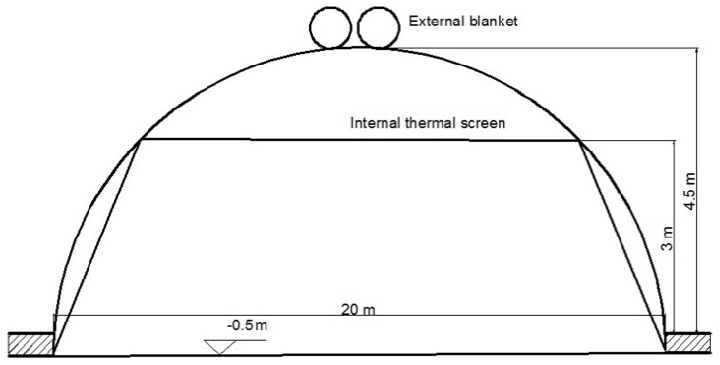
\includegraphics[width=11cm]{thrscr.png}
  \caption{Greenhouse thermal screen}\label{fig:thrscr}
\end{figure}

In figure~\ref{fig:thrscr}, we see that a thermal screen divides the green house into two compartments, above and below the screen.
This results in different concentrations of \(CO_2\) in two of the compartments.
\begin{figure}[H]
  \centering
  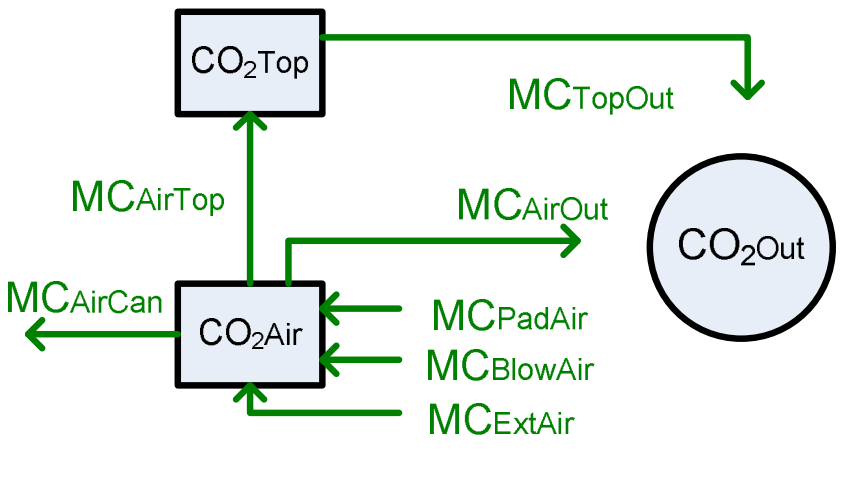
\includegraphics[width=9cm]{CO2}
  \caption{The \(CO_2\) flow inside and outside a greenhouse}\label{fig:CO2}
\end{figure}

The exchange in concentrations of \(CO_2\) can be separated into three \(CO_2\) region: \(CO_{2Top}\) which is from above the screen, \(CO_{2Air}\) which is from below the screen and \(CO_{2Out}\) which is from outside the greenhouse.
Each relates to each other in the diagram shown in figure~\ref{fig:CO2}.

%%%%%%%%%%
\subsubsection{Dynamical systems and assumptions}
From figure~\ref{fig:CO2}, the fluctuation of \(CO_2\) concentration in the lower and upper compartments of the greenhouse is represented by two differential equations.
\begin{align}
  \begin{cases}
    cap_{CO_2Air}\dot{CO_{2Air}} = MC_{BlowAir} + MC_{ExtAir} + MC_{PadAir} \\ \qquad \qquad \qquad \qquad \qquad
    - MC_{AirCan} - MC_{AirTop} - MC_{AirOut}                               \\
    cap_{CO_2Top}\dot{CO_{2Top}} = MC_{AirTop} - MC_{TopOut}
  \end{cases}
\end{align}

The notations \(cap_A, CO_{2 A}, \dot{CO_2}_A\) and \(MC_{AB}\) are respectively the capacity to store \(CO_2\) in \(A\) (\(m\)), the \(CO_2\) concentration in \(A\) (\(mg\;m^{-3}\)), the rate of change of \(CO_2\) concentration in \(A\) (\(mg\;m^{-3}\;s^{-1}\)), and the net \(CO_2\) flux from \(A\) to \(B\) (\(mg\;m^{-2}\;s^{-1}\)), where \(Air\) and \(Top\) represent the lower and upper compartments, \(Blow\) represents the direct air heater, \(Ext\) represents the source from the third party, \(Pad\) represents the pad system, \(Can\) represents the total foliage of the plants inside the greenhouse, and \(Out\) represents the space outside the greenhouse.

In order to solve the equations, we must consider the formulas that calculate each \(MC_{AB}\) that was presented.

The amount of \(CO_2\) going from the direct air heater into the greenhouse air is given by taking the product of the capacity \(P_{Blow}\) (\(W\)) of the heater, the amount of \(CO_2\) generated for each Joule of sensible heat released by the heater \(\eta_{HeatCO_2}\) (\(mg_{CO_2}\;J^{-1}\)), and the dimensionless parameter \(U_{Blow}\), then dividing it by the area of the greenhouse \(A_{Flr}\) (\(m^2\)).
\begin{align}
  MC_{BlowAir} = \frac{\eta_{HeatCO_2}U_{Blow}}{A_{Flr}}
\end{align}

Similarly, the amount of \(CO_2\) that is pumped into the greenhouse by the third party equals the third party's ability to pump \(CO_2\) \(\phi_{ExtCO_2}\) (\(mg\;s^{-1}\)) times the dimensionless parameter \(U_{ExtCO_2}\), then divided by the area of the greenhouse.
\begin{align}
  MC_{ExtAir} = \frac{U_{ExtCO_2}\phi_{ExtCO_2}}{A_{Flr}}
\end{align}

The amount of \(CO_2\) that enters the greenhouse through the pad system is calculated differently.
It depends on the difference between the concentration of \(CO_2\) inside and outside the greenhouse, and the ability of the pad system for the air to go through.
As the pad can be adjusted to let more air in, the flux of the pad \(f_{Pad}\) (\(m^{-1}\)) can be given as the product of the permeability of the pad \(U_{Pad}\) and the ability for the airflow to pass through \(\phi_{Pad}\) (\(m^3\;s^{-1}\)) divided by the area of the greenhouse floor.
\begin{equation}
  \begin{split}
    MC_{PadAir} & = f_{Pad} (CO_{2 Out} - CO_{2 Air}) \\
    & = \frac{U_{Pad} \phi_{Pad}}{A_{Flr}} (CO_{2 Out} - CO_{2 Air})
  \end{split}
\end{equation}

The net flux of \(CO_2\) from the lower compartment to the upper compartment of the greenhouse is more complicated.
It depends on the difference in temperature and air density between the two compartments and the airflow rate through the thermal screen \(f_{ThScr}\) (\(m\;s^{-1}\)).
\begin{align}
  MC_{AirTop} = f_{ThScr} (CO_{2 Air} - CO_{2 Top})
\end{align}

Furthermore, \(f_{ThScr}\) is given by
\begin{align}
  f_{ThScr} = U_{ThScr} K_{ThScr} |T_{Air} - T_{Top}| ^{\frac{2}{3}} + (1 - U_{ThScr}) {\left[\frac{g(1 - U_{ThScr})W}{2\rho^{Mean}_{Air}} |\rho_{Air} - \rho_{Top}|\right]}^{\frac{1}{2}}
\end{align}

To calculate the the airflow rate, we consider the screen and the open regions separately, with \(U_{ThScr} \in [0,1]\) representing the percentage of places that are covered by the thermal screen. The flux through the screen depends on the difference between the temperature above and below the screen and the permeability of the screen \(K_{ThScr}\) (\(m\;K^{-\frac{2}{3}}\;s^{-1}\)).

At places that are not covered by the thermal screen, the flux is given by a Navier-Stokes equation depending on the difference of the air density below the screen \(\rho_{Air}\) and the air density above the screen \(\rho_{Top}\) (\(kg\;m^{-3}\)). \(W\) (\(m\)) is width of the thermal screen.

The net \(CO_2\) flux from the inside to the outside of the greenhouse is given by the following formula
\begin{align}
  MC_{AirOut} = (f_{VentSide} + f_{VentForced})(CO_{2 Air} - CO_{2 Out})
\end{align}

The flux \(f_{VentSide}\) and \(f_{VentForced}\) (\(m s^{-1}\)) are respectively the flux due to the fan system on the sidewalls and the fan system inside the greenhouse.

%In this case, we should consider the Bernoulli principle in representing the pressure difference outside and inside of the greenhouse.

\begin{multline}
  \label{eq:vent_roof_side}
  f_{VentRoofSide} = \frac{C_d}{A_{Flr}} \biggl[\frac{U_{Roof}^2 U_{Side}^2 A_{Roof}^2 A_{Side}^2}{U_{Roof}^2 A_{Roof}^2 + U_{Side}^2 A_{Side}^2} \cdot \frac{2gh_{SideRoof} (T_{Air} - T_{Out})}{T_{Air}^{Mean}} \\
    + \biggl(\frac{U_{Roof} A_{Roof} + U_{Side} A_{Side}}{2}\biggr)^2 + C_W v_{Wind}^2\biggr]^{\frac{1}{2}}
\end{multline}

The above formula is the sum of the two components multiplied with the ratio between the discharged coefficient \(C_d\) and the area of the greenhouse \(A_{Flr}\) (\(m^2\)).

The first component represents the Stack effect when the ventilation area on the roof \(A_{Roof}\) (\(m^2\)) is non-zero. Stack effect happens when there exists a temperature difference between the interior and exterior of the building. In this case, the first component in the formula is given based on the equation of the Stack effect, that is caused by the temperature difference between the outside and inside of the greenhouse (the space under the thermal screen).
The second component is given by the pressure difference inside and outside the greenhouse. The pressure from the outside of the greenhouse is caused by the natural airflow through the roof surface, while the pressure from the inside of the greenhouse is caused by the lateral airflow. Based on the Bernoulli principle, the pressure difference can be calculated as the total area of the ventilation openings on the greenhouse divided by two times the natural wind speed \(v_{Wind}\) (\(m\;s^{-1}\)) squared and the global wind pressure coefficient \(C_w\) (dimensionless).

In the presence of an insect screen, the movement speed of the air currents through the ventilation areas will be reduced by a factor of \(\eta_{InsScr}\), where \(\zeta_{InsScr}\) is the porosity, the ratio of the area of the holes in the screen to the total area of the screen.
\begin{align}
  \eta_{InsScr} = \zeta_{InsScr} (2 -  \zeta_{InsScr})
\end{align}

Given the leakage coefficient \(c_{leakage}\), which depends on the greenhouse type and is dimensionless, an amount of approximately half the leakage rate is added to the air-exchange rate, where leakage rate is calculated as below.
\begin{align}
  f_{leakage} = \begin{cases}
    0.25 \cdot c_{leakage}     & \text{if~} v_{Wind} < 0.25    \\
    v_{Wind} \cdot c_{leakage} & \text{if~} v_{Wind} \geq 0.25
  \end{cases}
\end{align}

Let \(\eta_{Side\_Thr}\) be the Stack-effect threshold. If \(\eta_{Side}\), the ratio between the sidewalls ventilation
area and the total ventilation area, exceeds the threshold, the Stack effect does not occur and vice versa. Then, \(f_{VentSide}\) is given by the following
\begin{gather}
  f_{VentSide} =
  \begin{cases}
    \eta_{InsScr} f''_{VentSide} + 0.5f_{leakage} & \text{if~} \eta_{Side} \geq \eta_{Side\_Thr} \\
    \begin{split}
      & \eta_{InsScr} [U_{ThScr}f''_{VentSide} + \\
      & (1-U_{ThScr})f_{VentRoofSide} \eta_{Side}] + 0.5 f_{leakage}
    \end{split}                    & \text{if~} \eta_{Side} < \eta_{Side\_Thr}
  \end{cases}
\end{gather}

In which,  \(f''_{VentSide}\) is  \(f_{VentSide}\) when \(A_{Roof} = 0\).
Moreover, the Stack effect does not occur where is covered by the thermal screen.

The flux \(f_{VentForced}\) by the fan system inside the greenhouse is calculated as follows.
\begin{align}
  f_{VentForced} = \frac{\eta_{InsScr} U_{VentForced} \phi_{VentForced} } {A_{Flr}}
\end{align}

The dimensionless parameter \(U_{VentForced} \in [0,1]\) is to adjust the wind speed \(\phi_{VentForced}\) due to
the system (\(m^3\;s^{-1}\)).

Similarly to \(MC_{AirOut}\), the net \(CO_2\) flux from the greenhouse to outside the greenhouse through the roof openings is calculated by using the formula below, where \(f_{VentRoof}\) is the flux rate through the roof openings.
\begin{align}
  MC_{TopOut} = f_{VentRoof}(CO_{2 Top} - CO_{2 Out})
\end{align}

\(f_{VentRoof}\) is the flux rate openings and is given by
\begin{gather}
  f_{VentRoof} =
  \begin{cases}
    \eta_{InsScr} f''_{VentRoof} + 0.5f_{leakage} & \text{if~} \eta_{Roof} \geq \eta_{Roof\_Thr} \\
    \begin{split}
      & \eta_{InsScr} [U_{ThScr}f''_{VentRoof} + \\
      & (1-U_{ThScr})f_{VentRoofSide} \eta_{Side}] + 0.5 f_{leakage}
    \end{split}                    & \text{if~}  \eta_{Roof} < \eta_{Roof\_Thr}
  \end{cases}
\end{gather}

% check again part
However, when the ratio of the roof-opening area to the total ventilation area exceeds the Stack-effect threshold, the Stack effect does not occur and we cannot reuse the formula~\eqref{eq:vent_roof_side} where \(A_{Side} = 0\) to
calculate \(f''_{VentRoof}\).
\begin{align}
  f''_{VentRoof} = \frac{C_d U_{Roof} A_{Roof}}{2A_{Flr}} {\left[\frac{gh_{Roof}(T_{Air} - T_{Out})}{2T^{Mean}_{Air}} + C_w v^2_{Wind}\right]}^{ \frac{1}{2}}
\end{align}

Finally, we need to consider the amount of \(CO_2\) absorbed into the leaves due to photosynthesis.
\begin{align}
  MC_{AirCan} = M_{CH_2O} h_{C_{Buf}} (P - R)
\end{align}

Here, \(M_{CH_2O}\) is the molar mass of \(CH_2O\) (\(mg\;\mu mol^{-1}\)), \(P\) is the photosynthetic rate (\(\mu mol_{CO_2}\;m^{-2}\;s{-1}\)), \(R\) is the respiration rate (\(\mu mol_{CO_2}\;m^{-2}\;s^{-1}\)), and \(h_{C_{Buf}}\) shows the cessation of photosynthesis when \(CH_2O\) is \(C_{Buf}\) (\(mg\;m^{-2}\)) has reached \(C_{Max}\) (\(mg\;m^{-2}\)), which is the limit of the carbohydrates storage of the plants. The respiration rate during this process is usually as about \(1\%\) of the photosynthesis rate, and thus can be omitted during further calculation. The photosynthesis rate is described in more detail in Section~\ref{sssec:photo_c3}.

%%%%%%%%%%%
\subsubsection{A model of photosynthesis of C3 plants}\label{sssec:photo_c3}
Photosynthesis, the process by which green plants and certain other organisms transform light energy into chemical energy. During photosynthesis in green plants, light energy is captured and used to convert water, carbon dioxide, and minerals into oxygen and energy-rich organic compounds.

Photosynthesis has two phases: light-dependent phase and light-independent (or dark) phase.

The photosynthetic rate \(P\) is defined as the diffusion of \(CO_2\) from air into the leaf cells through stomata. From Fick's law for gas diffusion, we construct:
\begin{align}
  \label{eq:photo_co2}
  P = \frac{CO_{2Air} - CO_{2Stom}}{Res}
\end{align}

The notation \(CO_{2Stom}\) is the concentration of \(CO_2\) in the stomata (\(\mu mol\;m^{-3}\)) and \(Res\) is the resistance-to-absorption coefficient (\(s\;m^{-1}\)).

This way of calculating photosynthetic rate \(P\) is different from the model of Vanthoor 2011. In there the author uses:
\begin{align}
  P = \frac{J \cdot (CO_{2Stom} - \Gamma)}{4 \cdot (CO_{2Stom} + 2\Gamma)}
\end{align}
where \(J\) (\(\mu mol \{e^-\} m^{-2} s^{-1}\)) is the electron transport rate, 4 (\(\mu mol \{e^-\} \mu mol^{-1} \{CO_2\}\)) is the
number of electrons per fixed \(CO_2\) molecule, \(CO_{2Stom}\) (\(\mu mol\{CO_2\}\;mol^{-1}\{air\}\)) is the \(CO_2\) concentration in the stomata and \(\Gamma\) (\(\mu mol \{CO_2\} mol^{-1} \{air\}\)) is the \(CO_2\) compensation point.

Following by the photorespiration \(R\):
\begin{align}
  R = P \cdot \frac{\Gamma}{CO_{2Stom}}
\end{align}

But since we do not consider electron transport rate, we will use equation~\eqref{eq:photo_co2} constructed from Fick's law combined with Michaelis-Menten model.

In the dark phase, through Michaelis-Menten relationship describing enzyme-substrate reaction, the photosynthetic rate is given by:
\begin{align}
  \label{eq:photo_dark}
  P = \frac{P_{Max} \cdot CO_{2Stom}}{CO_{2\;0.5} + CO_{2Stom}}
\end{align}
where \(CO_{2\;0.5}\) is the concentration of \(CO_2\) in the substrate when \(P = P_{Max}/2\) (\(\mu mol\;m^{-3}\)).

From~\eqref{eq:photo_co2} and~\eqref{eq:photo_dark}, we form a quadratic equation for the rate of photosynthetic \(P\). The photosynthetic rate \(P\) then no longer depends on the concentration of \(CO_2\) in the stomata but only on the concentration of \(CO_2\) in the air, the resistance coefficient \(Res\), and the maximum photosynthetic rate.
\begin{align}
  \label{eq:resist_photo}
  ResP^2 - (CO_{2Air} + CO_{2\;0.5} + ResP_{Max})P + CO_{2Air}P_{Max} = 0
\end{align}

Solving equation~\eqref{eq:resist_photo} requires \(P_{Max}\) to be obtained. For the model for the photosynthesis of one leaf unit, the maximum photosynthetic rate is usually be found through the Arrhenius model.
\begin{align}
  \label{eq:photo_rate}
  k(T) = k(T_0)\exp \left(-\frac{H_a}{R} \left(\frac{1}{T} - \frac{1}{T_0}\right)\right)
\end{align}
where \(k(T)\) is the reaction rate at \(T(K)\), \(T_0\) is the optimum temperature for which the reaction
rate is known (\(K\)), \(H_a\) is the activation energy for the reaction (\(J\;mol^{-1}\)), and \(R\) is the ideal gas constant.

Yet a problem is raised when the temperature increases to a certain threshold, the enzyme activity will be inhibited and the photosynthesis is slowed down and cease to advance. A model represents the activity of the Rubisco enzyme during photosynthesis with temperature as its parameter.
\begin{align}
  \label{eq:rubisco}
  f(T) = \frac{1 + \exp \left(-\frac{H_d}{R} \left(\frac{1}{T_0} - \frac{1}{\frac{H_d}{S}}\right)\right)}{1 + \exp \left(-\frac{H_d}{R}\left(\frac{1}{T} - \frac{1}{\frac{H_d}{S}}\right)\right)}
\end{align}
In the model~\eqref{eq:rubisco}, \(f(T)\) represents the enzyme activity at \(T(K)\), \(H_d\) is the deactivation energy (\(J\;mol^{-1}\)), and \(S\) is the corresponding entropy quantity (\(J\;mol^{-1}\;K^{-1}\)).

Combining~\eqref{eq:photo_rate} and~\eqref{eq:rubisco}, we obtain the formula for maximum rate of photosynthetic rate.
\begin{align}
  \label{eq:photo_max}
  P_{Max}(T) = k(T)f(T)
\end{align}

For a photosynthesis for the whole canopy, considering \(LAI\) (leaf area index), due to Beer's law, the intensity of the transmitted beam \(I\) with the initial state is \(I_0\) (\(\mu mol\{photons\}\;m^{-2}\;s^{-1}\)) is equal to
\begin{align}
  I = \frac{I_0 \cdot K \cdot \exp \left(-K \cdot LAI\right)}{1 - m}
\end{align}

If the leaves are horizontally stratified such as in the case of tomato, the dimensionless extinction coefficient \(K\) will be between 0.7 and 1.0. Meanwhile, if the leaves are sloped as in the case of wet rice, \(K\) will be between 0.3 and 0.5. \(m\) is the transmittance coefficient of the leaves which is set as \(0.1\).

The amount of light absorbed by the canopy can be measured as the difference in the intensity of the light ray before entering the foliage and after passing through the foliage
\begin{align}
  L =L_0 \left(1 - \frac{K \cdot \exp \left(-K \cdot LAI\right)}{1 - m}\right)
\end{align}

In this formula, \(L\) is luminous flux received by the leaves per unit area of the greenhouse floor (\(\mu mol\{photons\}\;m^{-2}\;s^{-1}\)) and \(L_0\) is the initial value of \(L\).

For calculating the maximum photosynthetic rate of all leaves in the greenhouse, we apply the modified Arrhenius model.
\begin{align}
  \label{eq:photo_rate_mod}
  k(T) = LAI \cdot k(T_0) \cdot \exp \left(-\frac{H_a}{R} \left(\frac{1}{T} - \frac{1}{T_0}\right)\right)
\end{align}

Here, \(k(T)\) is the reaction rate for the whole canopy at \(T(K)\) and \(k(T_0)\) is the reaction rate under the optimal condition \(T_0\) \(K\) of one leaf unit.

Unlike the photosynthesis model for one leaf unit, the amount of light energy absorbed into the foliage in response to \(LAI\) needs to be added since it affects the maximum photosynthetic rate \(P_{Max}\). Therefore, we consider the following formula of \(P_{Max}\), which is a dependent function on \(L\) and \(T\).
\begin{align}
  P_{Max} (L,T) = \frac{P_{MLT} \cdot P_{Max}(T) \cdot L}{L + L_{0.5}}
\end{align}

In which, \(L_{0.5}\) is light intensity when \(P_{Max} (L,T) = P_{Max}(T)/2\) (\(\mu mol\{photons\}\;m^{-2}\;s^{-1}\))
\(P_{Max}(T)\) is calculated by using the formula~\eqref{eq:photo_max} with \(k(T)\) as in~\eqref{eq:photo_rate_mod}, and \(P_{MLT}\) are the maximum
photosynthetic rate at the point of light saturation and the optimal temperature \(T\).

\subsubsection{Vanthoor 2011 model of photosynthesis}
For calculating photosynthesis rate and respiration rate, we implement through the photosynthesis model described in Vanthoor 2011.

The photosynthesis rate is calculated through:
\begin{align}
  P = \frac{J \cdot (CO_{2Stom} - \Gamma)}{4 \cdot (CO_{2Stom} + 2\Gamma)}
\end{align}
where \(J\) (\(\mu mol\{e^-\}\;m^{-2}\;s^{-1}\)) is the electron transport rate, \(4\) (\(\mu mol \{e^-\} \; \mu mol^{-1} \{CO_2\}\)) is the number of electrons per fixed \(CO_2\) molecule, \(CO_{2Stom}\) (\(\mu mol\{CO_2\}\;mol^{-1}\{air\}\)) is the \(CO_2\) concentration in the stomata and \(\Gamma\) (\(\mu mol \{CO_2\}\; mol^{-1} \{air\}\)) is the \(CO_2\) compensation point.

Following by the photorespiration \(R\):
\begin{align}
  R = P \cdot \frac{\Gamma}{CO_{2Stom}}
\end{align}

The electron transport rate, J, is a function of the potential rate of electron transport and of the absorbed \(PAR\) by the canopy:

\begin{align}
  J = \frac{J^{POT} + \alpha PAR_{can} - {\sqrt{(J^{POT} + \alpha PAR_{can})}^2 - 4\Theta\cdot J^{POT}\cdot \alpha PAR_{can}}}{2 \Theta}
\end{align}
where \(J^{POT}\) (\(\mu mol\{e^-\}\;m^{-2}\;s^{-1}\)) is the potential rate of electron transport, \(PAR_{Can}\) (\(PAR\) by the canopy) (\(\mu mol\{photons\}\;m^{-2}\;s^{-1}\)) is the absorbed \(PAR\), \(\alpha\) (\(\mu mol\{e^-\}\;\mu mol^{-1}\{photons\}\)) is the conversion factor from photons to electrons, including an efficiency term, and \(\Theta\) (\(-\)) is the degree of curvature of the electron transport rate.

The potential rate of electron transport \(J^{POT}\), depends on temperature:

\begin{align}
  J^{POT} = J^{MAX}_{25,Can} \cdot \exp \left(E_j\frac{T_{Can,K}-T_{25,K}}{R\cdot T_{Can,K}\cdot T_{25,K}}\right) \cdot \frac{1 + \exp \left(\frac{S\cdot T_{25,K}-H}{R\cdot T_{25,K}}\right)}{1 + \exp \left(\frac{S\cdot T_{Can,K}-H}{R\cdot T_{Can,K}}\right)}
\end{align}
where \(J^{MAX}_{25,Can}\) (\(\mu mol \{e^-\}\;m^{-2}\;s^{-1}\)) is the maximum rate of electron transport at \(25 \degree C\) for the canopy, \(E_j\) (\(J\;mol^{-1}\)) is the activation energy for \(J^{POT}\), \(T_{Can,K}\) (\(K\)) is the canopy temperature, \(T_{25,K}\) (\(K\)) is the reference temperature at \(25 \degree C\), \(R\) (\(J\;mol^{-1}\;K^{-1}\)) is the molar gas constant, \(S\) (\(J\;mol^{-1}\;K^{-1}\)) is the entropy term and \(H\) (\(J\;mol^{-1}\)) is the deactivation energy.

The maximum rate of electron transport at \(25 \degree C\) for the canopy is calculated by:
\begin{align}
  J^{MAX}_{25,Can} = LAI \cdot J^{MAX}_{25,Leaf}
\end{align}
where \(J^{MAX}_{25,Leaf}\), (\(\mu mol\{e^-\}\;m^{-2}\{leaf\}\;s^{-1}\)) is the maximum rate of electron transport for the leaf at \(25 \degree C\).

The total \(PAR\) absorbed by the canopy is the sum of the \(PAR\) transmitted by the greenhouse cover that is directly absorbed, and the \(PAR\) reflected by the greenhouse floor that is indirectly absorbed:
\begin{align}
  PAR_{Can} = PAR_{GhCan} + PAR_{FlrCan}
\end{align}

The \(PAR\) which is directly absorbed by the canopy is described by a negative exponential decay of light with \(LAI\) in a homogeneous crop:
\begin{align}
  PAR_{GhCan} = PAR_{Gh}\cdot (1-\rho_{can})\cdot(1 - \exp \left(-K_1\cdot LAI\right))
\end{align}
where \(PAR_{Gh}\) (\(\mu mol \{photons\}\;m^{-2}\;s^{-1}\)) is the \(PAR\) above the canopy, \(\rho_{can}\) (\(-\)) is the reflection coefficient of the canopy for \(PAR\) and \(K_1\) is the extinction coefficient of the canopy for \(PAR\) (\(-\)).

The PAR above the canopy is described by:
\begin{align}
  PAR_{Gh} = \tau_{Gh} \cdot \eta_{Glob\_PAR}\cdot I_{Glob}
\end{align}
where \(\tau_{Gh}\) (\(-\)) is the light transmission of the greenhouse cover \(\eta_{Glob\_PAR}\) (\(\mu mol\{photons\}\;J^{-1}\)) is a conversion factor from global radiation to \(PAR\) and \(I_{Glob}\) (\(W\;m^{-2}\)) is the outside global radiation.

Absorption of \(PAR\) reflected by the greenhouse floor is described by:
\begin{align}
  PAR_{FlrCan} = \rho_{Flr}PAR_{Gh}\cdot (1-\rho_{Can})\cdot \exp \left(K_1\cdot LAI\right) \cdot (1 - \exp \left(K_2\cdot LAI\right))
\end{align}
where \(\rho_{Flr}\) (\(-\)) is the reflection coefficient of the greenhouse floor and \(K_2\) (\(-\)) is the extinction coefficient of the canopy when \(PAR\) is reflected from the floor to the canopy. We assumed \(K_2\) to be equal to \(K_1\).

The \(CO_2\) concentration inside the stomata, \(CO_{2Stom}\) depends on the stomatal and mesophyll conductance, boundary layer resistance, the photosynthesis rate and the difference between the \(CO_2\) concentration in the stomata and the \(CO_2\) concentration of the greenhouse air. However, the \(CO_2\) concentration in the stomata is assumed to be a fixed fraction of the \(CO_2\) concentration in the greenhouse air:
\begin{align}
  CO_{2Stom} = \eta_{CO_{2Air\_Stom}} \cdot CO_{2Air}
\end{align}
where \(\eta_{CO_{2Air\_Stom}}\) is conversion factor from the \(CO_2\) concentration of the greenhouse air, \(CO_{2Air}\), to the \(CO_2\) concentration in the stomata.

The \(CO_2\) compensation point (\(\Gamma\)) affects the leaf photosynthesis rate and depends on temperature. To avoid unrealistically low optimal canopy temperatures, the sensitivity of the compensation point to temperature was adjusted by making the slope dependent of the ratio of \(J^{MAX}_{25,Leaf}\) and \(J^{MAX}_{25,Can}\):
\begin{align}
  \Gamma = \frac{J^{MAX}_{25,Leaf}}{J^{MAX}_{25,Can}}c_{\Gamma} T_{Can} + 20 c_{\Gamma}(1-\frac{J^{MAX}_{25,Leaf}}{J^{MAX}_{25,Can}})
\end{align}
where \(c_{\Gamma}\) (\(\mu mol\{CO2\}\;mol^{-1}\{air\}\;K^{-1}\)) determines the effect of canopy temperature on the \(CO_2\) compensation point. The right term of the equation above is introduced to assure that, for all values of \(J^{MAX}_{25,Can}\) at a temperature of \(20 \degree C\).

\subsection{Implementing the programs}
% TODO


\newpage
%%%%%%%%%%%%%%%%%%%%%%%%%%%%%%%%%
\section{Testing the programs}
% TODO


\newpage
%%%%%%%%%%%%%%%%%%%%%%%%%%%%%%%%%
\section{Exercise 4}
\subsection{Euler and Runge-Kutta of order 4 algorithms as computer programs}
% TODO

\subsection{Predicting \(CO_2\) concentration and comparing to actual data}
% TODO


\newpage
%%%%%%%%%%%%%%%%%%%%%%%%%%%%%%%%%
\section{A dynamical system for vapor pressure}
\subsection{A vapor pressure model}
In this section, a dynamical system representing the vapor pressure in the greenhouse will be addressed.
The model was based on the following assumption:
1.\ the greenhouse air is considered to be a ``perfectly stirred tank'', meaning that there are no spatial differences in temperature, vapor pressure and the \(CO_2\) concentration; thus all the model fluxes are described per square metre of greenhouse floor;
2.\ to describe the effect of the thermal screen on the indoor climate, the greenhouse air was divided into two compartments: one below and one above the thermal screen.

\begin{figure}[H]
  \centering
  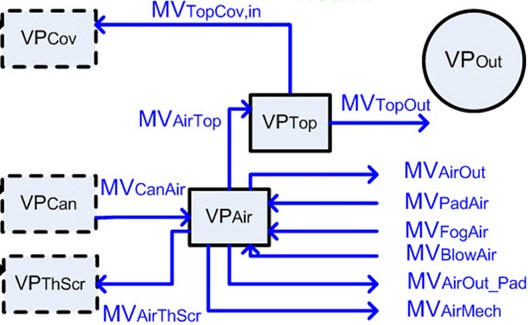
\includegraphics[width=0.6\textwidth]{VP}
  \caption{The vapor flow inside and outside a greenhouse}\label{fig:VP}
\end{figure}

The exchange in vapor pressure can be separated into three regions: \(VP_{Top}\) which is from above the screen, \(VP_{Air}\) which is from below the screen, and \(VP_{Out}\) which is from outside the greenhouse.
Their relation can be expressed as in figure~\ref{fig:VP}.

\subsection{Dynamical systems and assumptions}
The vapor pressure of the greenhouse air \(VP_{Air}\) is described by:
\begin{multline*}
  cap_{VP_{Air}}\dot{VP_{Air}} = MV_{CanAir} + MV_{PadAir} + MV_{FogAir} + MV_{BlowAir} \\
  - MV_{AirThScr} - MV_{AirTop} - MV_{AirOut} \\
  - MV_{AirOut\_Pad} - MV_{AirMech} ~~~~ [kg\;m^{-2}\;s^{-1}]
\end{multline*}
where \(cap_{VP_{Air}}\) is the capacity of the air to store water vapor.
Vapor is exchanged between the air and surrounding elements i.e.\ the canopy \(MP_{CanAir}\), the outlet air of the pad \(MV_{PadAir}\), the fogging system \(MV_{FogAir}\), the direct air heater \(MV_{BlowAir}\), the thermal screen \(MV_{AirThScr}\), the top compartment air \(MV_{AirTop}\), the outdoor air \(MV_{AirOut}\), the outdoor air due to the air exchange caused by the pad and fan system \(MV_{AirOut\_Pad}\), and the mechanical cooling system \(MV_{AirMech}\).

The vapor pressure of the air in the top compartment \(VP_{Top}\) is described by:
\begin{multline*}
  cap_{VP_{Top}}\dot{VP_{Top}} = MV_{AirTop} - MV_{TopCov,in} - MV_{TopOut} ~~~~~~~~~~~~~~~~~~~~~~~~~~~~ [kg\;m^{-2}\;s^{-1}]
\end{multline*}
where \(cap_{VP_{Top}}\) is the capacity of the top compartment to store water vapor, \(MV_{TopCov,in}\) is the vapor exchange between the top compartment and the internal cover layer, and \(MV_{TopOut}\) is the vapor exchange between the top compartment and the outside air.

The vapor exchange coefficient between the air and an object is linearly related to the convective heat exchange coefficient between the air and the object.
Therefore, the vapor flux from the air to an object by condensation is described by:
\begin{align}
  \label{eq:vapor_conden}
  MV_{12} = \begin{cases}
    0                                       & \text{if~} VP_1 < VP_2 \\
    6.4 \cdot 10^{-9} HEC_{12}(VP_1 - VP_2) & \text{if~} VP_1 > VP_2 \\
  \end{cases}
\end{align}
where \(MV_{12}\) (\(kg\;m^{-2}\;s^{-1}\)) is the vapor flux from air of location 1 to object 2, \(6.4 \cdot 10^{-9}\) is the conversion factor relating the heat exchange coefficient (\(W\;m^{-2}\;K^{-1}\)) to the vapor exchange coefficient (\(kg\;m^{-2}\;s^{-1}\;Pa^{-1}\)), \(HEC_{12}\) (\(W\;m^{-2}\;K^{-1}\)) is the heat exchange coefficient between the air of location 1 to object 2 and \(VP_1\) (\(Pa\)) is the vapor pressure of the air of location 1 and \(VP_2\) is the saturated vapor pressure of object 2 at its temperature.

Because this model should consist of only differentiable functions, equation~\eqref{eq:vapor_conden} was smoothed to:
\begin{align}
  MV_{12} = \frac{1}{1 + \exp \left(s_{MV_{12}} (VP_1 - VP_2)\right)} \cdot 6.4 \cdot 10^{-9} HEC_{12} (VP_1 - VP_2)
\end{align}
where \(s_{MV_{12}}\) (\(-\)) is the slope of the differentiable switch function for vapor pressure differences.

% AirThScr
The vapor flux from the greenhouse air compartment to the thermal screen and the vapor flux from the top compartment to the interval cover layer are described analogously to equation~\eqref{eq:vapor_conden}:
\begin{align}
  MV_{AirThScr}  & = \begin{cases}
    0                                                       & \text{if~} VP_{Air} < VP_{ThScr} \\
    6.4 \cdot 10^{-9} HEC_{AirThScr}(VP_{Air} - VP_{ThScr}) & \text{if~} VP_{Air} > VP_{ThScr} \\
  \end{cases} \\
  % TopCov,in
  MV_{TopCov,in} & = \begin{cases}
    0                                                         & \text{if~} VP_{Top} < VP_{Cov,in} \\
    6.4 \cdot 10^{-9} HEC_{TopCov,in}(VP_{Top} - VP_{Cov,in}) & \text{if~} VP_{Top} > VP_{Cov,in} \\
  \end{cases}
\end{align}
whereby their associated heat change coefficients are:
\begin{align}
  HEC_{AirThScr}  & = 1.7 U_{ThScr} |T_{Air} - T_{ThScr}|^{0.33}                        \\
  HEC_{TopCov,in} & = {c_{HECin} (T_{Top} - T_{Cov,in})}^{0.33} \frac{A_{Cov}}{A_{Flr}}
\end{align}
with \(U_{ThScr} \in [0,1]\) representing the percentage of places that are covered by the thermal screen, \(T_X\) (\(\degree C\)) is the temperature at location \(X\), \(c_{HECin}\) (\(W\;m^{-2}\;K^{-2}\)) is the convective heat exchange parameter between cover and outdoor air depending on the greenhouse shape, \(A_{Cov}\) (\(m^2\)) is the surface of the cover including the side-walls, and \(A_{Flr}\) (\(m^2\)) is the surface of the greenhouse floor.

The general form of a vapor flux accompanying an air flux is described by:
\begin{align}
  \label{eq:vapor_air}
  MV_{12} = \frac{M_{Water}}{R} f_{12} \left(\frac{VP_1}{T_1 + 273.15} - \frac{VP_2}{T_2 + 273.15}\right)
\end{align}
where \(MV_{12}\) (\(kg\;m^{-2}\;s^{-1}\)) is the vapor flux from location 1 to location 2, \(f_{12}\) (\(m^3\;m^{-2}\;s^{-1}\)) is the air flux from location 1 to location 2, \(T_1\) and \(T_2\) (\(\degree C\)) are the temperature at location 1 and 2 respectively.

% AirTop
The vapor fluxes from the air compartment to the top compartment, the air compartment to the outdoor air, and the top compartment to the outdoor air are described analogously to equation~\eqref{eq:vapor_air}:
\begin{align}
  MV_{AirTop} & = \frac{M_{Water}}{R} f_{ThScr} \left(\frac{VP_{Air}}{T_{Air} + 273.15} - \frac{VP_{Top}}{T_{Top} + 273.15}\right)                       \\
  % AirOut
  MV_{AirOut} & = \frac{M_{Water}}{R} (f_{VentSide} + f_{VentForced}) \left(\frac{VP_{Air}}{T_{Air} + 273.15} - \frac{VP_{Out}}{T_{Out} + 273.15}\right) \\
  % TopOut
  MV_{TopOut} & = \frac{M_{Water}}{R} f_{VentRoof} \left(\frac{VP_{Top}}{T_{Top} + 273.15} - \frac{VP_{Out}}{T_{Out} + 273.15}\right)
\end{align}

% CanAir
The canopy transpiration is described by:
\begin{align}
  MV_{CanAir} = VEC_{CanAir}(VP_{Can} - VP_{Air})
\end{align}
where \(VEC_{CanAir}\) (\(kg\;Pa\;s^{-1}\)) is the vapor exchange coefficient between the canopy and air, \(VP_{Can}\) is the saturated vapor pressure at canopy temperature.

According to Stanghellini (1987), the vapor transfer coefficient of the canopy transpiration can be calculated by:
\begin{align}
  VEC_{CanAir} = \frac{2 \rho_{Air} c_{p,Air}LAI}{\Delta H \gamma (r_b + r_s)}
\end{align}
where \(\rho_{Air}\) (\(kg\;m^{-3}\)) is the density of the greenhouse air, \(c_{p,Air}\) (\(J\;K^{-1}\;kg^{-1}\)) is the specific heat capacity of the greenhouse air, \(LAI\) (\(m^2\;m^{-2}\)) is the leaf area index, \(\Delta H\) (\(J\;kg^{-1}\)) is the latent head of evaporation of water, \(\gamma\) (\(Pa\;K^{-1}\)) is the psychometric constant, \(r_b\) (\(s\;m^{-1}\)) is the boundary layer resistance of the canopy for vapor transport and \(r_s\) (\(s\;m^{-1}\)) is the stomatal resistance of the canopy for vapor transport.

The boundary layer resistance for vapor transport depends on the wind speed in the greenhouse and the temperature difference between the canopy and surrounding air (Stanghellini, 1987).
However, the wind speed in the greenhouse is not measured nor simulated and therefore a constant boundary layer resistance was used.
The stomatal resistance of the canopy is described by a simplification of the stomatal resistance model of Stanghellini (1987):
\begin{align}
  r_s = r_{s,\min} \cdot rf(R_{Can}) \cdot rf(CO_{2Air\_ppm}) \cdot rf(VP_{Can} - VP_{Air})
\end{align}
where \(r_{s,\min}\) (\(s\;m^{-1}\)) is the minimum canopy resistance and \(rf\) is the resistance factor for high radiation levels, high \(CO_2\) levels and large vapor pressure differences.
The resistance factors are described according to Stangellini (1987):
\begin{equation*}
  \begin{split}
    & rf(R_{Can}) = \frac{R_{Can} + c_{evap1}}{R_{Can} + c_{evap2}} \\
    & rf(CO_{2Air}) = 1 + {c_{evap3} (\eta_{mg\_ppm} CO_{2Air} - 200)}^2 \\
    & rf(VP_{Can} - VP_{Air}) = 1 + {c_{evap4} (VP_{Can} - VP_{Air})}^2
  \end{split}
\end{equation*}
where \(R_{Can}\) (\(W\;m^{-2}\)) is the global radiation above the canopy, \(c_{evap1}\) (\(W\;m^{-2}\)), \(c_{evap2}\) (\(W\;m^{-2}\)), \(c_{evap3}\) (\(ppm^{-2}\)), \(c_{evap4}\) (\(Pa^{-2}\)) are empirically determined parameters and \(\eta_{mg\_ppm}\) (\(ppm\;mg^{-1}\;m^3\)) is the conversion factor from \(mg\;m^{-3}\;CO_2\) to \(ppm\).
Stanghellini limited the resistance factor for high \(CO_2\) levels to 1.5 and the resistance factor for large vapor pressure differences to 5.8 and determined the transpiration variables \(c_{evap3}\) and \(c_{evap4}\) for day time and night time.
The values of the transpiration parameters \(c_{evap3}\) and \(c_{evap4}\) differed between the night period and day period which means that the accompanying equations are not differentiable at sunrise and sunset. Therefore the parameters \(c_{evap3}\) and \(c_{evap4}\) were smoothed using the differentiable switch function:
\begin{align}
  S_{r_s} = \frac{1}{1 + \exp \left(s_{r_s} (R_{Can} - R_{Can\_SP})\right)}
\end{align}
where \(S_{r_s}\) (\(-\)) is the value of the differentiable switch, \(s_{r_s}\) (\(m\;W^{-2}\)) is the slope of the differentiable switch for the stomatal resistance model and \(R_{Can\_SP}\) (\(W\;m^{-2}\)) is the radiation value above the canopy to define sunrise and sunset.
Using the differential switch, the smoothed transpiration parameters were described by:
\begin{align}
  c_{evap3} & = c_{evap3}^{night} (1 - S_{r_s}) + c_{evap3}^{night} S_{r_s} \\
  c_{evap4} & = c_{evap4}^{night} (1 - S_{r_s}) + c_{evap4}^{night} S_{r_s}
\end{align}

% BlowAir
The vapor flux from the heat blower to the greenhouse air is proportional to the head flux:
\begin{align}
  MV_{BlowAir} = \eta_{HeatVap} H_{BlowAir}
\end{align}
where \(\eta_{HeatVap}\) (\(kg\{vapor\}\;J^{-1}\)) is the amount of vapor which is released when 1 Joule of sensible energy is produced by the direct air heater.

% PadAir
The vapor flux from the pad and fan to the greenhouse air is described by:
\begin{align}
  MV_{PadAir} = \rho_{Air} f_{Pad} (\eta_{Pad} (x_{Pad} - x_{Out}) + x_{Out})
\end{align}
where \(f_{Pad}\) (\(m^3\;m^{-2}\;s^{-1}\)) is the ventilation flux due to the pad and fan system, \(\eta_{Pad}\) (\(-\)) is the efficiency of the pad and fan system, \(x_{Pad}\) (\(kg\{water\} kg^{-1}\{air\}\)) is the water vapor content of the pad and \(x_{Out}\) (\(kg\{water\} kg^{-1}\{air\}\)) is the water vapor content of the outdoor air.

The ventilation flux due to the pad and fan system is desribed by:
\begin{align}
  f_{Pad} = \frac{U_{Pad} \phi_{Pad}}{A_{Flr}}
\end{align}
where \(U_{Pad}\) (\(-\)) is the control valve of the pad and fan system and \(\phi_{Pad}\) (\(m^3\;s^{-1}\)) is the capacity of the air flux through the pad.

% AirOut_Pad
The vapor flux from the greenhouse air to the outside air when using the pad and fan system is described by:
\begin{align}
  MV_{AirOut\_Pad} = f_{Pad} \frac{M_{Water}}{R} \left(\frac{VP_{Air}}{T_{Air} + 273.15}\right)
\end{align}

% AirMech
The vapor flux from the greenhouse air to the surface of mechanical cooling system is described analogously to equation~\eqref{eq:vapor_conden}:
\begin{align}
  MV_{AirMech} = \begin{cases}
    0                                                     & \text{if~} VP_{Air} < VP_{Mech} \\
    6.4 \cdot 10^{-9} HEC_{AirMech}(VP_{Air} - VP_{Mech}) & \text{if~} VP_{Air} > VP_{Mech} \\
  \end{cases}
\end{align}
with \(HEC_{AirMech}\) is the heat exchange coefficient between the greenhouse air and the surface of the mechanical cooling unit:
\begin{align}
  HEC_{AirMech} = - \frac{U_{MechCool} COP_{MechCool} P_{MechCool} / A_{Flr}}{T_{Air} - T_{MechCool} + 6.4 \cdot 10^{-9} \Delta H(VP_{Air} - VP_{MechCool})}
\end{align}
where \(U_{MechCool}\) (\(-\)) is the control valve of the mechanical cooling mechanism, \(COP_{MechCool}\) (\(-\)) is the coefficient of performance of the mechanical cooling system and \(P_{MechCool}\) is the electrical capacity of the mechanical cooling system, \(T_{MechCool}\) (\(\degree C\)) is the temperature of the cooling surface, and \(VP_{MechCool}\) (\(Pa\)) is the saturated vapor pressure of the mechanical cooling mechanism.

% FogAir
The latent head flux from the greenhouse air depends on the vapor flux from the fogging system to the greenhouse air which is described by:
\begin{align}
  MV_{FogAir} = \frac{U_{Fog} \phi_{Fog}}{A_{Flr}}
\end{align}
where \(U_{Fog}\) (\(-\)) is the control valve of the fogging system and \(\phi_{Fog}\) (\(kg\{water\}\;s^{-1}\)) is the capacity of the fogging system.

% TODO: Implement programs

\subsection{Testing the programs}
% TODO

\subsection{Predicting vapor pressure and comparing to actual data}
% TODO


\newpage
%%%%%%%%%%%%%%%%%%%%%%%%%%%%%%%%%
\section{Exercise 6}
\subsection{(a)}
% TODO

\subsection{(b)}
% TODO

\subsection{(c)}
% TODO

\begin{thebibliography}{80}
  \bibitem{bib1}
  % TODO


  \bibitem{bib2}
  % TODO


\end{thebibliography}
\end{document}

